\documentclass[12pt]{article}

%===============================
%
%          📦 Paquetes
%
%===============================

\usepackage[a4paper, top=2cm, bottom=2cm, left=2.5cm, right=2.5cm]{geometry}
\usepackage[spanish,es-noshorthands]{babel}
\usepackage[utf8]{inputenc}
\usepackage[table]{xcolor}
\usepackage{amsmath}
\usepackage{multicol}
\usepackage{graphicx}
\usepackage{hyperref}
\usepackage{booktabs}
\usepackage{pgfplots}
\pgfplotsset{compat=1.18}
\usepackage{tikz}

\title{
  \vspace{2cm}
  \pagenumbering{gobble}
  
\includegraphics[width=5cm]{../assets/logo-utp.png} \\
  \vspace{1cm}
  \textbf{Universidad Tecnológica del Perú} \\
  \vspace{2cm}
  \textbf{Cálculo I} \\
  \vspace{1cm}
  \large \textbf{Portafolio de Actividades}
}
\author{
  \textbf{Torres Vara, Mateo Nicolas} - \texttt{U24308542} \\
  \texttt{Sección 32384}
}



\begin{document}
\maketitle
\begin{center}

  Docente: Victor Johnny Papuico Bernardo

\end{center}

%======================================
%
%          📚 Inicio del documento
%
%======================================

\newpage
\section*{Actividad 1}
\noindent Realice una reflexión sobre las propiedades: Resistencia, Reciclable, Reutilizable,
Degradable y Eficiente de un envase de leche en lata de una empresa que opere en nuestro
país.

\begin{itemize}
    \item \textbf{Resistencia:} La resistencia de un envase de leche en lata es fundamental para garantizar la protección del producto. Debe ser capaz de soportar condiciones de transporte y almacenamiento sin deformarse ni romperse.
    \item \textbf{Reciclable:} Es importante que el material del envase sea reciclable para minimizar el impacto ambiental. Las latas de aluminio, por ejemplo, son altamente reciclables y pueden ser reutilizadas para fabricar nuevos productos.
    \item \textbf{Reutilizable:} Aunque las latas de leche en sí no son reutilizables, es posible fomentar la reutilización a través de programas de devolución o incentivos para que los consumidores devuelvan las latas vacías.
    \item \textbf{Degradable:} Si bien las latas de metal no son biodegradables, es esencial que los envases alternativos, como los de cartón, sean diseñados para descomponerse de manera segura en el medio ambiente.
    \item \textbf{Eficiente:} La eficiencia en el diseño del envase puede contribuir a la reducción de residuos y al uso óptimo de recursos. Esto incluye la minimización del material utilizado y la optimización del espacio en el transporte.
\end{itemize}




\newpage
\section*{Actividad 2}
\noindent Usted como ingeniero debe diseñar un protector de cartón para una barra de mantequilla con las siguientes especificaciones: \\

\vspace{-0.5cm}

\begin{center}
  \begin{tabular}{r|l}
    \begin{tabular}{l}
      Espesor de la barra: 1,5cm \\
      Ancho de la barra: entre 4 y 6cm inclusive \\
      Largo de la barra: El triple del ancho disminuido en 4cm \\
    \end{tabular}
    &
    \(
    \begin{array}{l}
      h = 1.5\text{ cm} \\
      4 \leq w \leq 6\text{ cm} \\
      l = 3w - 4\text{ cm} \\
    \end{array}
    \) \\
  \end{tabular}
\end{center}

\begin{itemize}
  \item Represente una función en una variable que modele el área del cartón para este protector (elija una variable que se encuentre dentro de las condiciones dadas).
  \[
  \begin{array}{l}
    2(1.5)(w) + 2(1.5)(3w - 4) + 2(w)(3w - 4) \\\\
    3w + 9w - 12 + 6w^2 - 8w = 6w^2 + 4w - 12
  \end{array}
  \]
  \item Represente gráficamente la función del ítem anterior mediante la plataforma digital (GEOGEBRA, DESMOS, etc), indicando dominio y rango.
  \begin{center}
  \begin{tikzpicture}
    % Espesor(1.5) x Largo(3w-4)
    \draw (0,1.5) -- (1.5,1.5) -- (1.5,9.5) -- (0,9.5) -- cycle;
    \draw (5.5,1.5) -- (7,1.5)-- (7,9.5) -- (5.5,9.5) -- cycle;
    % Espesor(1.5) x Ancho(w)
    \draw (1.5,0) -- (1.5,1.5) -- (5.5,1.5) -- (5.5,0) -- cycle;
    \draw (1.5,9.5) -- (5.5,9.5) -- (5.5,11) -- (1.5,11) -- cycle;
    % Ancho(w) x Largo(3w-4)
    \draw (1.5,1.5) -- (5.5,1.5) -- (5.5,9.5) -- (1.5,9.5) -- cycle;
    \draw (7,1.5) -- (11,1.5) -- (11,9.5) -- (7,9.5) -- cycle;

    % Etiqueta de ancho
    \node[above] at (3.5,11) {w};
    % Etiquetas de espesor
    \node[left] at (1.4,10.25) {1.5cm};
    \node[left] at (1.4,0.75) {1.5cm};
    % Etiquetas de largo
    \node[rotate=90, above] at (0,5.5) {3w - 4cm};
  \end{tikzpicture}
  \end{center}
  \begin{center}
  \begin{tikzpicture}
    \begin{axis}[
      axis lines = left,
      xlabel = {Ancho de la barra $w$ (cm)},
      ylabel = {Área del cartón $A(w)$ ($cm^2$)},
      domain=4:6,
      samples=100,
      width=10cm,
      height=10cm,
      grid=both,
      minor tick num=1,
      every major grid/.style={gray, opacity=0.5},
      every minor grid/.style={gray, opacity=0.2},
      ymin=0,
      ymax=300,
      xmin=0,
      xmax=8,
      legend style={at={(0.97,0.97)},anchor=north east}
    ]
    % Curva de la función
    \addplot [
      thick,
      color=blue,
    ]
    {6*x^2 + 4*x - 12};
    \addlegendentry{$A(w) = 6w^2 + 4w - 12$}

    % Punto marcado
    \addplot[
      only marks,
      mark=*,
      color=red
    ] coordinates {(4,100) (6, 228)};
    \addlegendentry{Puntos $(4,\;100)$ y $(6,\;228)$}

    \end{axis}
  \end{tikzpicture}
  \end{center}
  \item Calcule la mínima cantidad de material que se puede usar en este protector.
  \[
    A(w) = 6w^2 + 4w - 12 = 6(4)^2 + 4(4) - 12 = 96 + 16 - 12 = 100cm^2
  \]
\end{itemize}





\newpage
\section*{Actividad 3}
\noindent Usted como ingeniero debe diseñar un envase de lata para una nueva presentación de la
empresa GLORIA, para ello debe analizar la presentación más vendida de la empresa (ver imagen)
\begin{center}
\begin{tikzpicture}[remember picture]
  \node[anchor=south west,inner sep=0] (img) at (0,0) {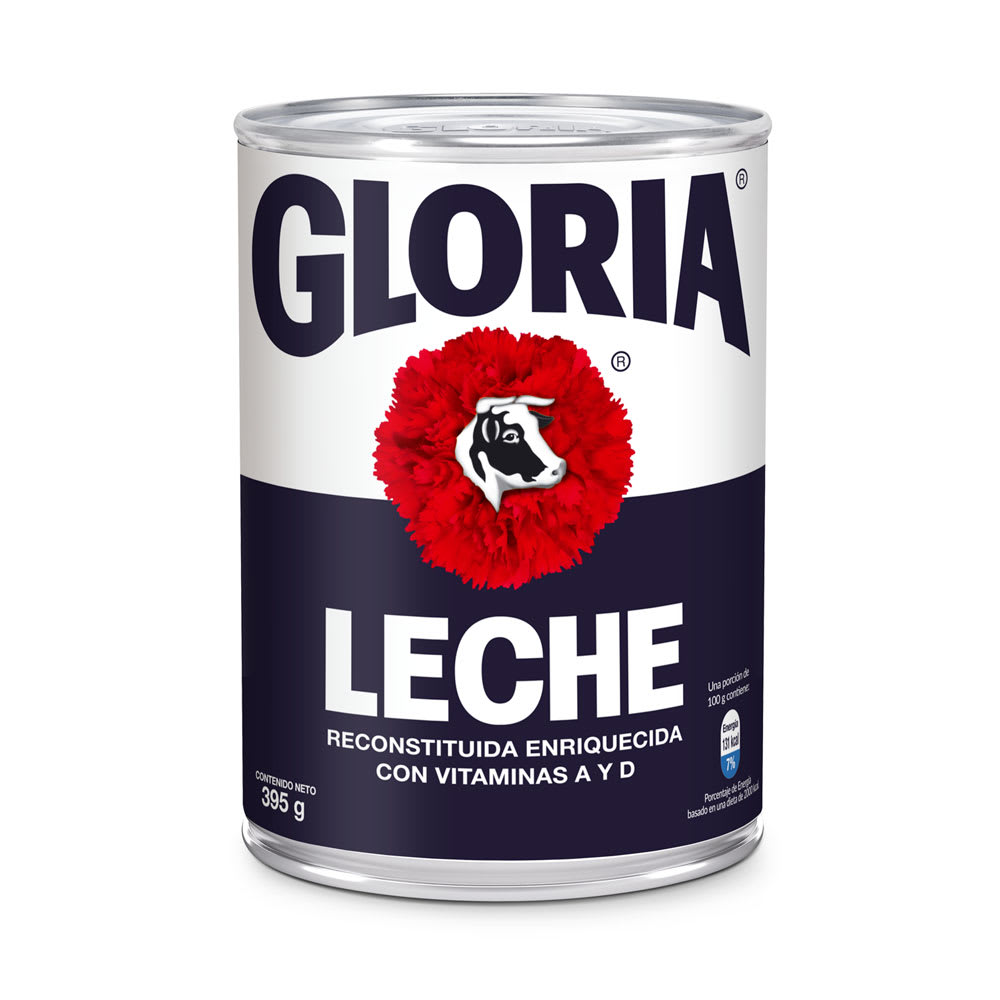
\includegraphics[width=0.7\textwidth]{./assets/leche-gloria.jpg}};
  \begin{scope}[x={(img.south east)},y={(img.north west)}]
    \draw (0.2,0.1) -- (0.2,0.9);
    \node [rotate=90, above] at (0.2,0.5) {10cm};

    \draw (0.23, 0.94) -- (0.77,0.94);
    \node [above] at (0.5,0.94) {7.5cm};
  \end{scope}
\end{tikzpicture}
\end{center}

\begin{itemize}
  \item Presente una imagen donde usted está midiendo el diámetro y altura del envase e 
  indique cuanto material (área total) se usó en su fabricación.
  \[
    A(h) = 2\pi r^2 + 2\pi rh = 2\pi (3.75)^2 + 2\pi (3.75)(10) = 88.36 + 235.62 = 323.98cm^2
  \]
  \item Usted como ingeniero recibe el encargo de diseñar un nuevo envase cilíndrico de
  capacidad 500ml, para ello debe presentar una función en una variable que
  represente la cantidad de material a usar en ese envase. Además, debe analizar la
  gráfica mediante la plataforma digital (GEOGEBRA, DESMOS, etc) e indicar las
  características de esa función. \textbf{Para este caso, $h=2r$}
  \vspace{-0.75cm}
  \begin{center}
    \[
    \begin{array}{l|l|l}
      \begin{array}{l}
        V = \pi r^2 h \implies h = \dfrac{V}{\pi r^2} \\\\
        A(r) = 2\pi r^2 + 2\pi r\left(\dfrac{V}{\pi r^2}\right) \\\\
        A(r) = 2\pi r^2 + \dfrac{2V}{r}
      \end{array}
      &
      \begin{array}{l}
        500 = 2\pi r^3 \\\\
        r^3 = \dfrac{500}{2\pi} \\\\
        r = \sqrt[3]{\dfrac{500}{2\pi}} \approx 4.30127cm
      \end{array}
      &
      \begin{array}{l}
        \pi r^2 h \\\\
        \pi \cdot 4.30127^2 \cdot 8.60254\\\\
        = 500ml
      \end{array}
    \end{array}
    \]
  \end{center}
  \begin{center}
    \begin{tikzpicture}
      \begin{axis}[
        axis lines = left,
        xlabel = $r$,
        ylabel = {$A(r)$},
        domain=1:10,
        samples=100,
        width=10cm,
        height=10cm,
        grid=both,
        minor tick num=1,
        every major grid/.style={gray, opacity=0.5},
        every minor grid/.style={gray, opacity=0.2},
        ymin=0,
        legend style={at={(0.97,0.97)},anchor=north east} % leyenda en esquina sup. der.
      ]
      % Curva de la función
      \addplot [
        thick,
        color=blue,
      ]
      {2*pi*x^2 + 1000/x};
      \addlegendentry{$A(r) = 2\pi r^2 + \tfrac{2V}{r}$}
  
      % Punto marcado
      \addplot[
        only marks,
        mark=*,
        color=red
      ] coordinates {(4.30127,348.73421)};
      \addlegendentry{Punto $(4.3013,\;348.7342)$}
  
      \end{axis}
    \end{tikzpicture}
  \end{center}
  \item Si el área técnica le informa que el nuevo envase cilíndrico presentará dos tipos
  de material (uno para el área lateral y otro para las bases), donde el material para el
  área lateral y bases presenta costos diferentes, según la información del cuadro:
  \begin{center}
    \begin{tabular}{c@{\hspace{2cm}}c}
      % ------- Primera tabla -------
      \begin{tabular}{|c|c|}
        \hline
        \multicolumn{2}{c}{\cellcolor{red!30}{Material para área lateral}} \\
        Calidad & Costo por $cm^2$ \\
        \hline
        Calidad 1 & $0,01$ \\
        Calidad 2 & $0,02$ \\
        Calidad 3 & $0,03$ \\
        Calidad 4 & $0,04$ \\
        Calidad 5 & $0,05$ \\
        \hline
      \end{tabular}
      &
      % ------- Segunda tabla -------
      \begin{tabular}{|c|c|}
        \hline
        \multicolumn{2}{c}{\cellcolor{red!30}{Material para las bases}} \\
        Calidad & Costo por $cm^2$ \\
        \hline
        Calidad 1 & $0,06$ \\
        Calidad 2 & $0,07$ \\
        Calidad 3 & $0,08$ \\
        Calidad 4 & $0,09$ \\
        Calidad 5 & $0,10$ \\
        \hline
      \end{tabular}
      \\\\
      % ------- Ecuaciones debajo -------
      \(
        \begin{aligned}
          \tfrac{2V}{r} \cdot 0.01 \\
          = \tfrac{1000}{4.30127}\cdot 0.01 \\
          = 2.3255
        \end{aligned}
      \)
      &
      \(
        \begin{aligned}
          2\pi r^2 \cdot 0.07 \\
          = 2\pi (4.30127)^2 \cdot 0.07 \\
          = 8.1271
        \end{aligned}
      \)
    \end{tabular}
  \end{center}
\end{itemize}





\newpage
\section*{Actividad 4}
\noindent Luego de su excelente desempeño en la empresa GLORIA, usted es contratado por la empresa 
FANNY para optimizar los costos de fabricación del envase de su producto más vendido (ver imagen)

\begin{center}
  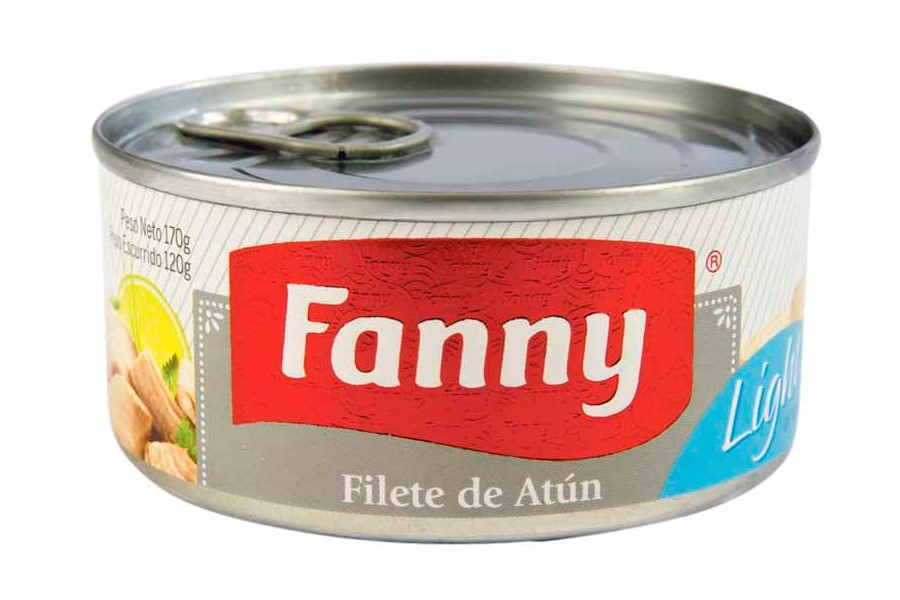
\includegraphics[width=0.8\textwidth]{./assets/fanny-filete.jpg}
\end{center}

\noindent Según el área comercial de la empresa los clientes piden una conserva que tenga 20\% más
de capacidad, para lo cual usted debe realizar lo siguiente:
\begin{itemize}
  \item Proponga la imagen de un nuevo envase cilíndrico. \textbf{Para este caso, $h=r$}
  \begin{center}
  \begin{tikzpicture}[scale=0.7]
    % Parámetros
    \def\radio{5} % Escala arbitraria para el radio
    \def\altura{5} % h = r

    % Cuerpo del cilindro
    \draw[thick] (0,0) ellipse ({\radio} and 1); % base inferior
    \draw[thick] (0,\altura) ellipse ({\radio} and 1); % base superior
    \draw[thick] (-\radio,0) -- (-\radio,\altura);
    \draw[thick] (\radio,0) -- (\radio,\altura);

    % Líneas ocultas de la base superior
    \draw[dashed] (0,\altura) +(-\radio,0) arc (180:360:{\radio} and 1);

    % Etiquetas
    \draw[<->] (\radio+0.5,0) -- (\radio+0.5,\altura) node[midway,right] {$h$};
    \draw[<->] (0,-1.2) -- (\radio,-1.2) node[midway,below] {$r$};

    % Valores numéricos
    \node at (0,-2) {$h = r$};
    \node at (0,-2.7) {$V = 600\,\text{cm}^3$};
  \end{tikzpicture}
  \end{center}

  \item Proponga costos diferentes para el material usado en el área lateral y en las bases.
  Se usará el material de calidad 3 para el área lateral y calidad 4 para las bases.

  \item Presente una función en una variable que modele el costo total del envase.
  \[
    \begin{array}{l}
      V = \pi r^2 h \implies h = \dfrac{V}{\pi r^2} \\\\
      A(r) = 2\pi r^2 + 2\pi r\left(\dfrac{V}{\pi r^2}\right) \\\\
      A(r) = 2\pi r^2 + \dfrac{2V}{r} \\\\
      C(r) = (0.03)(2\pi r^2) + (0.09)\left(\dfrac{2V}{r}\right) \\\\
      C(r) = 0.06\pi r^2 + \dfrac{0.18V}{r}
    \end{array}
  \]

  \item Grafique la función mediante la plataforma digital (GEOGEBRA, DESMOS, etc).
  \begin{center}
  \begin{tikzpicture}
    \begin{axis}[
      axis lines = left,
      xlabel = $r$,
      ylabel = {$C(r)$},
      domain=1:20,
      samples=100,
      width=10cm,
      height=10cm,
      grid=both,
      minor tick num=1,
      every major grid/.style={gray, opacity=0.5},
      every minor grid/.style={gray, opacity=0.2},
      ymin=0,
      legend style={at={(0.97,0.97)},anchor=north east} % leyenda en esquina sup. der.
    ]
    % Curva de la función
    \addplot [
      thick,
      color=blue,
    ]
    {0.06*pi*x^2 + (0.18*600)/x};
    \addlegendentry{$C(r) = 0.06\pi r^2 + \tfrac{0.18V}{r}$}

    % Punto marcado
    \addplot[
      only marks,
      mark=*,
      color=red
    ] coordinates {(6.59221,24.57447)};
    \addlegendentry{Punto $(6.59221,\;24.57447)$}

    \end{axis}
  \end{tikzpicture}
  \end{center}
\end{itemize}


\end{document}